\documentclass[10pt]{article}
\usepackage[utf8]{inputenc}
\usepackage{mathtools}
\usepackage{amsmath}
\usepackage{graphicx}
\usepackage{array}
\usepackage[margin=0.5in]{geometry}
\usepackage{listings}
\usepackage{color}

\definecolor{mygreen}{rgb}{0,0.6,0}
\definecolor{mygray}{rgb}{0.5,0.5,0.5}
\definecolor{mymauve}{rgb}{0.58,0,0.82}

\lstset{ %
  backgroundcolor=\color{white},   % choose the background color; you must add \usepackage{color} or \usepackage{xcolor}; should come as last argument
  basicstyle=\footnotesize,        % the size of the fonts that are used for the code
  breakatwhitespace=false,         % sets if automatic breaks should only happen at whitespace
  breaklines=true,                 % sets automatic line breaking
  captionpos=b,                    % sets the caption-position to bottom
  commentstyle=\color{mygreen},    % comment style
  deletekeywords={...},            % if you want to delete keywords from the given language
  escapeinside={\%*}{*)},          % if you want to add LaTeX within your code
  extendedchars=true,              % lets you use non-ASCII characters; for 8-bits encodings only, does not work with UTF-8
  frame=single,	                   % adds a frame around the code
  keepspaces=true,                 % keeps spaces in text, useful for keeping indentation of code (possibly needs columns=flexible)
  keywordstyle=\color{blue},       % keyword style
  language=Octave,                 % the language of the code
  morekeywords={*,...},            % if you want to add more keywords to the set
  numbers=left,                    % where to put the line-numbers; possible values are (none, left, right)
  numbersep=5pt,                   % how far the line-numbers are from the code
  numberstyle=\tiny\color{mygray}, % the style that is used for the line-numbers
  rulecolor=\color{black},         % if not set, the frame-color may be changed on line-breaks within not-black text (e.g. comments (green here))
  showspaces=false,                % show spaces everywhere adding particular underscores; it overrides 'showstringspaces'
  showstringspaces=false,          % underline spaces within strings only
  showtabs=false,                  % show tabs within strings adding particular underscores
  stepnumber=2,                    % the step between two line-numbers. If it's 1, each line will be numbered
  stringstyle=\color{mymauve},     % string literal style
  tabsize=2,	                   % sets default tabsize to 2 spaces
  title=\lstname                   % show the filename of files included with \lstinputlisting; also try caption instead of title
}
\renewcommand{\arraystretch}{1.5}
\setcounter{secnumdepth}{0}
\author{Kevin Mambu}
\date{\today}
\title{M1 SESI 2017-2018\\Architecture Multi-Processeurs\\TP6 : Interruptions
vectorisées \\ Communications avec les périphériques}

\begin{document}
\maketitle

\section{A) Objectifs}
Le but de ce TP est d’analyser les mécanismes de communication par interruptions
entre les périphériques et le système d'exploitation. Dans une première partie
de ce TP, on illustre sur une architecture bi-processeurs le mécanisme des
interruptions vectorisées en utilisant un Timer programmable, capable de générer
des interrutions périodiques. Dans une seconde partie, on analyse en détail le
mécanisme permettant à un programme de lire des catactères à partir d'un terminal
TTY.
\newline
On dit qu'un périphérique est "mappé" en mémoire lorsqu'il possède des
registres adressables par le logiciel (au moyen d’instructions de lecture ou
d’écriture du type lw ou sw).

\begin{itemize}
  \item Les registres accessibles en écriture permettent au système
  d'exploitation de configurer les périphériques, ou de leur envoyer des
  commandes.
  \item Les registres accessibles en lecture permettent au système
  d'exploitation d'obtenir des informations sur l'état du périphérique.
\end{itemize}

Pour communiquer avec le système d'exploitation, les périphériques utilisent des
interruptions : Une interruption, ou IRQ (Interrupt ReQuest) est un signal
booleen actif à l'état haut, qui permet à à un périphérique de "voler " quelques
cycles à un processeur pour exécuter une ISR (Interrupt Service Routine). Ces
ISR ont généralement pour rôle d'écrire dans des tampons mémoire appartenant au
système d'exploitation. Ces tampons de communication sont spécifiques pour
chaque type de périphérique.
\newline
L’architecture matérielle est identique à l'architecture matérielle définie pour
le TP5, mais on utilisera seulement deux processeurs.

\section{B) Architecture matérielle}
\begin{center}
  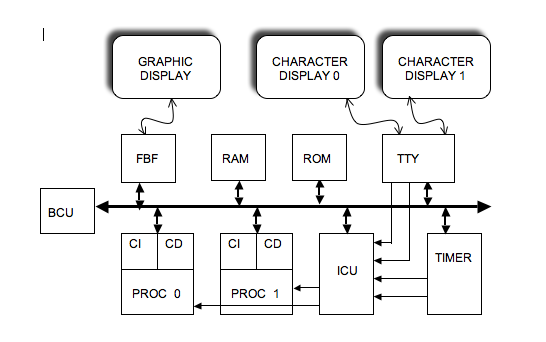
\includegraphics[width=14cm]{tp6_topcell.png}
\end{center}

\section{C) Composants périphériques}
{\it Les spécifications sont en annexe}

\subsection{Question C1}
Le composant {\bf PibusMultiTimer} est une cible et non un maître sur le bus
parce que :
\begin{itemize}
  \item Elle n'émet pas de données sur le bus indépendamment d'une requête
  de la cible.
  \item Toute emission d'interruption (TIMER\_IRQ) est en réalité à la demande
  du système d'exploitation.
\end{itemize}
{\bf PibusMultiTimer} est d'avantage un contrôleur de timers indépendants :
\texttt{ntimer} est le nombre de timers indépendants sous {\bf PibusMultiTimer}.
\newline
{\it Regarder l'annexe des spécifications pour les registres adressables et
leurs offsets par rapport à l'adresse de base du segment SEG\_TIMER\_BASE}

\subsection{Question C2}
Le composant {\bf PibusMultiTimer} est une cible et non un maître sur le bus
parce que :
\begin{itemize}
  \item Elle n'émet pas de données sur le bus indépendamment d'une requête
  de la cible.
  \item Même si à la suite de la sortie de l'ICU, \texttt{IRQ\_OUT}, un accès
  mémoire est fait (lecture/écriture de registres), cela est la conséquence
  de l'ISR associée à l'interruption et exécutée par le processeur.
  \item Et elle est également dépendante du système d'exploitation.
\end{itemize}
\texttt{nirq} est le nombre de signaux d'interruptions branchés sur l'ICU (cela
indique par conséquence le nombre de périphériques sur l'architecture).
\newline
L'ICU du PIBUS est un contrôleur multi-canaux, \texttt{nproc} indique le nombre
de processeurs reliés à l'ICU et ainsi le nombre de sorties IRQ\_OUT.
\newline
L'ICU est un contrôleur reprogrammable. Lors du boot, le code du reset a parmi
ses tâches d'effectuer le routage interne de l'ICU des requêtes entrantes
IRQ\_IN[\texttt{nirq}] vers IRQ\_OUT[\texttt{nproc}]. Le système d'exploitation
peut également impacter sur le routage interne.
\newline
Soit n l'identifiant du processeur au sein de l'architecture vis-à-vis de l'ICU
et l'adresse de base du segment SEG\_ICU\_BASE, chaque processeur est associé à
un sous-segment dont l'adresse de base est $SEG\_ICU\_BASE + n \times 5$. Les
offsets et les fonctionnalités de chaque registe sont décrits dans l'annexe.

\subsection{Question C3}
L'adresse de base de l'ICU SEG\_ICU\_BASE doit être alignée multiple de $32
\times 8$ octets parce que chaque proceseur lui est attribué 5 registres, soit
20 octets, qu'on rehausse à 32 par souci d'alignement. Relâcher cette
contrainte aurait pour conséquence de limiter le nombre de sous-canaux
correctement utilisables, car l'un d'entre eux n'aurait pas de mapping mémoire
suffisant pour ses registres.

\subsection{Question C4}
Rappelons que nous sommes sur une architecture bi-processeurs ($\texttt{NPROC}
=2$).
\begin{itemize}
  \item IRQ\_IN[0] $\rightarrow$ DMA
  \item IRQ\_IN[1] $\rightarrow$ IOC
  \item IRQ\_IN[2+2i] $\rightarrow$ TIMER[i]
  \item IRQ\_IN[3+2i] $\rightarrow$ TTY[i], soit :
  \item IRQ\_IN[3] $\rightarrow$ TTY[0]
  \item IRQ\_IN[5] $\rightarrow$ TTY[1]
  \item IRQ\_IN[2] $\rightarrow$ TIMER[0]
  \item IRQ\_IN[4] $\rightarrow$ TIMER[1]
\end{itemize}

\section{D) Lancement des tâches}

\subsection{Question D2}
\begin{center}
  \begin{tabular}{|c|c|}
    \hline
    {\it main\_prime} & {\it main\_pgcd} \\ \hline
    \texttt{0x004012dc} & \texttt{0x004013f0} \\ \hline
  \end{tabular}
\end{center}

\subsection{Question D3}
Le flag de GCC, \texttt{freestanding} permet d'assumer que le début du programme
principal ne sera pas nécessairement à l'adresse \texttt{main}. L'option
\texttt{no-gpopt} demande à GCC de ne pas utiliser de pointeur global vers le
segment seg\_data. De ce fait, GCC utilise le mécanisme d'accès de labélisation
des données, ce qui nous fait notre table de saut.

\subsection{Question D4}
Le programme ne peut pas notifier de l'entrée d'un caractère car le processeur
n'est pas connecté à l'ICU et donc ne peut pas acquitter de l'interruption.

\section{E) Activation du timer}

\subsection{Question E1}
Pour se brancher à l'ISR de l'interruption concernée $i$, le processeur passe
par le tableau interrupt\_vector, qui est une table de saut, puis saute à
l'adresse stockée à interrupt\_vector[i].
\newline
Séquence d'appels de fonctions jusqu'à isr\_timer :
\begin{itemize}
  \item Point d'entrée au GIET
  \item \texttt{r27 <= Cause register}
  \item \texttt{r26 <= \_cause\_vector}
  \item \texttt{r26 <= \&\_cause\_vector[XCODE]}
  \item \texttt{r26 <= \_cause\_vector[XCODE]}
  \item Branchement à l'adresse dans \texttt{r26} (\_int\_handler)
  \item Réservation d'espace sur la pile d'appel
  \item Sauvegarde de contexte (\texttt{r1-r31, HI, LO, EPC})
  \item Brancchement à la fonction C \texttt{\_int\_demux}, de irq\_handler.c
  \item Lecture du registre de l'ICU \_ICU\_IT\_VECTOR
  \item S'il n'y a pas d'interruption active (lecture retourne 32)
  $\rightarrow$ retour à \_irq\_handler, sinon...
  \item \texttt{isr <= \_interrupt\_vector[index]} (\_isr\_timer)
  \item Branchement à la routine \_isr\_timer
\end{itemize}

\subsection{Question E2}
\_isr\_timer gère les deux timers connectés respectivement aux processeurs 0 et
1. Plus précisément, pour un timer TIMER[id], il acquitte l'interruption du
timer puis affiche un message sur le TTY.

\subsection{Question E6}
Rappel, les signaux \texttt{sel\_xxx} dinstinguent quel est la cible du
processeur via le PIBUS à un cycle donné.
\begin{itemize}
  \item Le processeur 0 écrit la première valeur dans le vecteur d'interruption
  au cycle 52 {\it (rappel : le vecteur d'interruptions est situé à ce moment
  dans la ram, car faisant partie de \texttt{sys.bin})}.
  \item Le registre ICU\_MASK[0] est configuré au cycle 56.
  \item Le TIMER[0] est configuré au cycle 86.
\end{itemize}

\subsection{Question E7}
La première interruption du TIMER[0] est reçue au cycle 50093.

\subsection{Question E8}
\begin{tabular}{|c|p{4cm}|}
  \hline
  {\bf Cycle} & {\bf Évenement} \\ \hline
  100094 & Levée de l'interruption \texttt{TIMER\_IRQ[0]} \\ \hline
  100114 & Branchement sur le point d'entrée du GIET (0x80000180) \\ \hline
  100123 & Branchement sur \texttt{\_int\_handler (restore)} \\ \hline
  100258 & Branchement sur \texttt{\_int\_demux} \\ \hline
  100494 & Branchement sur \texttt{\_isr\_timer} \\ \hline
  104348 & Retour à \texttt{\_int\_demux} \\ \hline
  104354 & Retour à \texttt{\_int\_handler} \\ \hline
  104423 & Retour au programme utilisateur (\texttt{eret}) \\ \hline
\end{tabular}

\subsection{Question E9}
Le GIET est un système d'exploitation non-préemptif, en le sens qu'un processeur
exécutant une routine bloquante en mode système aura malgré tout ses
interruptions non-masquées, sauf si explicitement déclaré autrement.

\section{F) Activation des interruptions TTY}

\subsection{Question F1}
Si le mécanisme de communication par interruption n'était pas asynchrone, alors:
\begin{itemize}
  \item Dans un cas où le programme destinataire ne serait pas exécuté par le
  processeur alors que l'interruption serait levée par le TTY, l'interruption
  resterait pendante et le contrôleur de TTY serait alors bloqué jusqu'à
  acquittement de l'interruption. Or, il n'y a aucun destinataire pour acquitter.
\end{itemize}

\subsection{Question F2}
Suite d'appels pour lire une chaîne de caractères décimaux :
\begin{itemize}
  \item tty\_getw\_irq
  \begin{itemize}
    \item sys\_call(SYSCALL\_TTY\_READ\_IRQ,...
    \begin{itemize}
      \item syscall
    \end{itemize}
    \item tty\_putc
    \begin{itemize}
      \item sys\_call(SYSCALL\_TTY\_WRITE,...
      \begin{itemize}
        \item syscall
      \end{itemize}
    \end{itemize}
  \end{itemize}
\end{itemize}

\subsection{Question F3}
La fonction \_isr\_tty\_get est un wrapper de la fonction
\_isr\_tty\_get\_indexed[0]. Si le tampon \_tty\_get\_buf est plein au moment de
l'appel de \_isr\_tty\_get, alors la valeur précedemment contenue dans le tampon
ets supprimée.

\subsection{Question F4}
\begin{itemize}
  \item \_tty\_read\_irq récupère le contenu du tampon du TTY associé au
  processeur appelant, puis met la bascule \_tty\_get\_full à 0 (bascule
  positionnée à RESET).
  \item Cette fonction prend en argument l'adresse vers un tampon de reception
  et une longeur maximale de lecture.
  \item Si le tampon du TTY est vide, aucune donnée est copiée dans le tampon
  de reception et la fonction retourne 0.
  \item \texttt{tty\_id = \_task\_context\_array[(proc\_id*NB\_MAXTASKS + task\_id)*64 + 34]} :
  \begin{itemize}
    \item \_task\_context\_array est la table des contextes de tâches, déclarée
    dans \textit{\texttt{ctx\_handler.c}}.
    \item La macro \texttt{TASK\_CTXT\_SIZE} définit la taille d'un contexte de
    tâches, elle est égale à 64.
    \item On peut deviner que 34 correspond au déplacement nécessaire pour
    accéder au champ tty\_id d'un contexte de tâches.
  \end{itemize}
\end{itemize}

\subsection{Question F5}
\begin{itemize}
  \item Les caractères spéciaux traités sont :
  \begin{itemize}
    \item \texttt{LF (line feed)} : End Of Line, associé à la touche "Enter".
    \item \texttt{CR (carriage return)} : retour chariot, associé à la touche
    "Enter".
    \item \texttt{DEL} : Suppresion de caractère, associé à la touche "Suppr"
  \end{itemize}
  \item En cas de \textit{Decimal String Overflow}, la chaîne de caractères est
  annulée, la variable recevante est mise à 0, et la fonction retourne 0.
\end{itemize}

\subsection{Question F6}
\begin{itemize}
  \item L'attribut \texttt{volatile} permet d'assurer qu'une variable puisse
  être modifiée également depuis l'extérieur du programme. Dans notre cas,
  \_tty\_get\_buf et \_tty\_get\_full sont des registres manipulés également par
  le contrôleur de TTY.
  \item Ces registres sont rangés dans le segment \texttt{seg\_tty}.
  \item Ce segment doit être rangés en non-cachable car ces registres peuvent
  être modifiés indépendamment des processeurs (modifiés par le contrôleur de
  TTY).
\end{itemize}

\newpage

\lstinputlisting{reset.s}

\newpage

\lstinputlisting{PibusIcu.desc}
\newpage
\lstinputlisting{PibusMultiTimer.desc}
\newpage
\lstinputlisting{PibusMultiTty.desc}
\end{document}
\end{document}
